
\chapter{La réionisation} 
\label{sec:introreio}

%réionisation et non rayonnisation!
%\section{Observation -> la reionization}
%%\section{Théorie -> La reionization}
%
%
%Qu'est ce que c'est?
%
%fin des âges sombres
%apparition des première sources de rayonnement
%Pourquoi étudier la réionisation
%
%Dernier processus impactant l'ensemble de l'univers.
%Importance pour le "missing satellite problem"
%%le manque d'observations
%%la difficulté des observations



Nous avons vu dans le chapitre précédent que lors de la recombinaison, l'Univers est passé d'un état globalement ionisé à un état globalement neutre.
%De cette transition, qui a eu lieu a environ 380000 ans après le Bigbang, en a résulté L’émission du CMB.
Suite à cette étape, l'Univers était alors très homogène et ne disposait pas de source lumineuse, cette étape s'appelle les "âges sombres".
Sa dynamique était régie essentiellement par la lutte entre l'expansion et la gravitation et la compétition entre ces deux effets, couplée à de très légères perturbations observable dans les anisotropies du \ac{CMB} a menée à l'effondrement de certaines de ses parties.
Il faudra alors attendre plusieurs centaines de million d'années pour voir apparaître des surdensités de gaz suffisamment compactes pour former les première étoiles.
Ces premières sources lumineuses ont émis un puissant rayonnement ionisant qui a à nouveau séparé les protons et les électrons réunis lors de la recombinaison.
Il a fallu encore plusieurs centaines de millions d'années supplémentaires pour que les sources de rayonnement soient suffisamment nombreuses pour que leurs photons remplissent l'Univers, et le fasse passer d'un état majoritairement neutre, à un état à nouveau majoritairement ionisé.
Cette transition s'appelle l’époque de la réionisation et est représenté sur la figure \ref{fig:frise}.
Les premières étoiles se forment à des redshifts supérieurs à 50 et forment des bulles de gaz ionisé autour d'elles appelées régions HII.
Avec l’effondrement des structures, la formation stellaire augmente, les sources de rayonnement augmentent en nombre et en intensité.
Les bulles d'ionisation grossissent et d'autres apparaissent.
Petit à petit les bulles fusionnent (ont dit qu'elles percolent) et le régions HII grandissent.
La réionisation est finie à redshift $z\approx 6$ quand le rayonnement atteins les dernières régions neutres.

L'objectif de cette section est de présenter quelques unes des preuves observationnelles qui confirment que la réionisation a bien eu lieu.
Je présenterai également les grandes lignes des principes physiques en cours durant cette période.

%à l'apparition des premières des premières étoiles.
%L'Univers va alors subir un changement d'état majeur, puisque le rayonnement énergétique des premières étoiles va de nouveau ioniser le gaz.
%C'est l'époque de la réionisation.

%Du fait que l'univers était neutre, le rayonnement n’était pas en mesure de se propager librement.
%A la suite de l'émission du fond diffus cosmologique, commence une période appelée "les ages sombres".
%L'Univers est alors composé de gaz froid soumis principalement à deux forces : la gravité et l'expansion de l'Univers.
%Ces étoiles ont émis du rayonnement suffisamment énergétique pour arracher les électrons du gaz environnant.

%Dans cette section, je vais présenter quelques unes des preuve observationnelles de la réionisation. 

\begin{figure}
\centering
        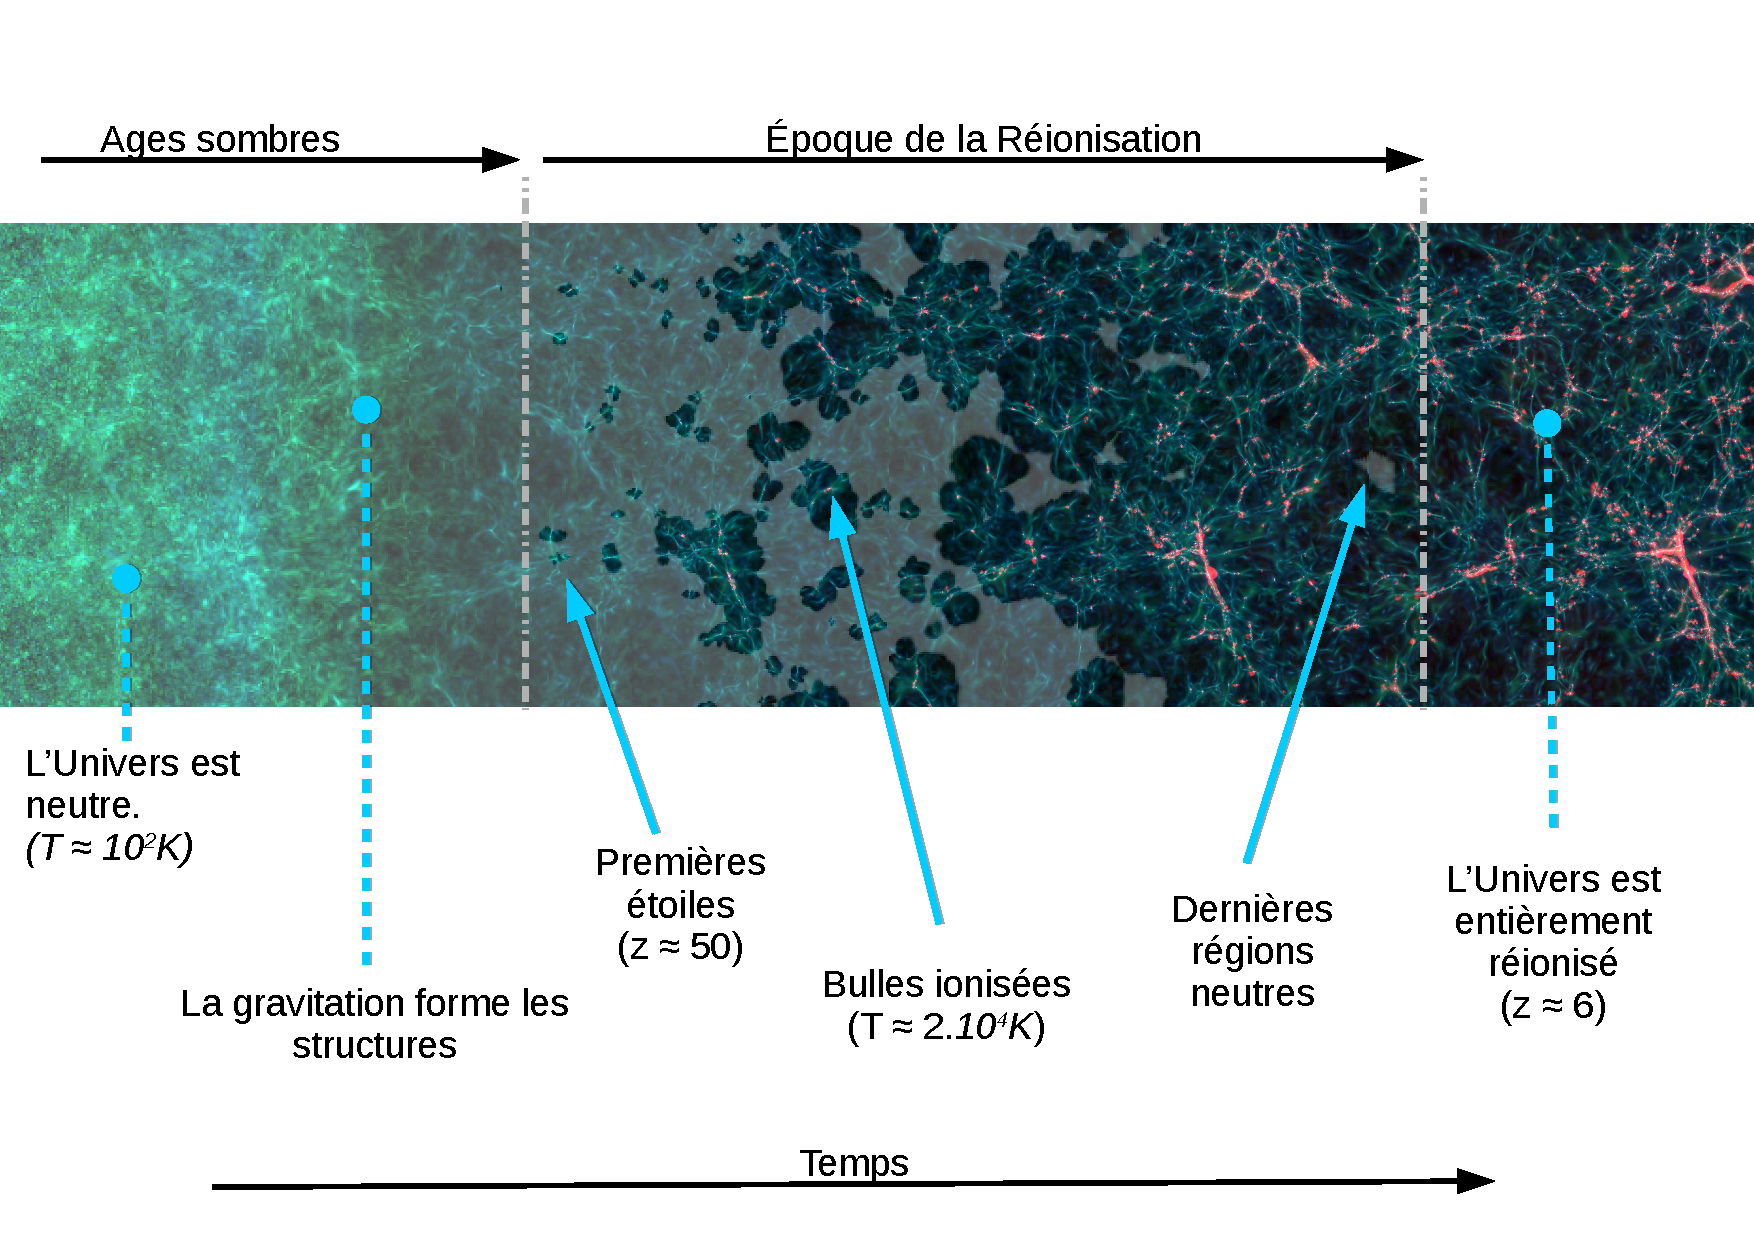
\includegraphics[width=\textwidth]{img/01/frise_legend.pdf} 
        \caption[Présentation de l'EoR]{Présentation de l'Époque de Réionisation. 
        L'apparition des premières étoiles introduit un rayonnement UV qui va petit à petit réioniser l'Univers.}
 		\label{fig:frise}
\end{figure}


\section{Preuves observationnelles}
\label{sec_contraintes_obs}

Dans cette section nous verrons quelles sont les principales observations en faveur de la réionisation de l'Univers.

\subsection{Spectres de quasars et épaisseur optique Lyman-alpha}

Historiquement, les spectres de quasars lointains ont été les premières preuves que l'Univers était majoritairement neutre dans le passé.
Les quasars sont des objets suffisamment brillants pour être observés à très grandes distances.
\cite{1965ApJ...141.1295S} observe que le spectre des plus lointains d'entre eux présentent une absorption caractéristique.
.%, appelée tunel Gun-Peterson \citep{1965ApJ...142.1633G}.
%Avant de poursuivre, il est nécessaire  de revenir sur le spectre d’émission de l’hydrogène.
%\subsubsection*{Raie Lyman alpha}
%\begin{figure}
%\centering
%        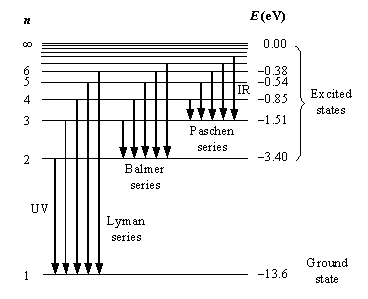
\includegraphics[width=.9\textwidth]{img/01/lyman.jpg} 
%        \caption[Raies de l'hydrogène]{Changement de niveau d'énergie de l'atome d'hydrogène}
% 		\label{fig:lyman}
%\end{figure}
%(cf Fig. \ref{fig:lyman}) 
%La série de Lyman correspond a la transition atomique menant au fondamental de l'atome d'hydrogène.
%Il existe plusieurs série de transition autre que celle de Lyman mais cette dernière est la plus énergétique et la plus fréquente, et donc la plus facile à détecter.
%Réciproquement, la transition n1 vers n2 mène a l'absorption d'un photon Lyman-alpha.

L'énergie de la raie Lyman-alpha, transition de l'électron du premier état excité vers l’état fondamental, est de 1216 $\AA$, ce qui place cette émission dans l'Ultra Violet.
Si un nuage de gaz neutre se trouve entre une source et l'observateur, le spectre réceptionné présentera une raie d'absorption à 1216 $\AA$.
Maintenant considéreront des distances cosmologiques entre la source et l'observateur.
Durant le parcours des photon, l'Univers aura subi une expansion et le spectre d'émission de la source sera décalé vers le rouge.
Le spectre présentera des raies d’absorptions à différents endroits suivant le moment de rencontre des différents nuages de gaz neutre.
C'est série de raies est très dense à haut redshift et est appelée forêt Lyman-alpha.
Maintenant, si la source est à l’intérieur d'une zone neutre, la série de raies absorbées ne sera plus discrète mais continue.
Ce continuum d’absorption est nommé tunnel Gunn-Peterson \citep{1965ApJ...141.1295S}
La figure \ref{fig:spectre_quasar} montre une série d'observations de spectres de quasars, classés par redshift.
Le tunnel Gunn-Peterson des plus éloignés est particulièrement visible.

%Dans le cas de la reionisation, les sources sont des quasar.
%Les quasars sont des objets suffisamment brillants pour être observé a très grandes distance.
%Il est observé que plus leur redshift est important, plus leur foret lyman alpha est important.
%Les plus lointains d'entre eux présentent  un tunnel gun peterson.

\begin{figure}
        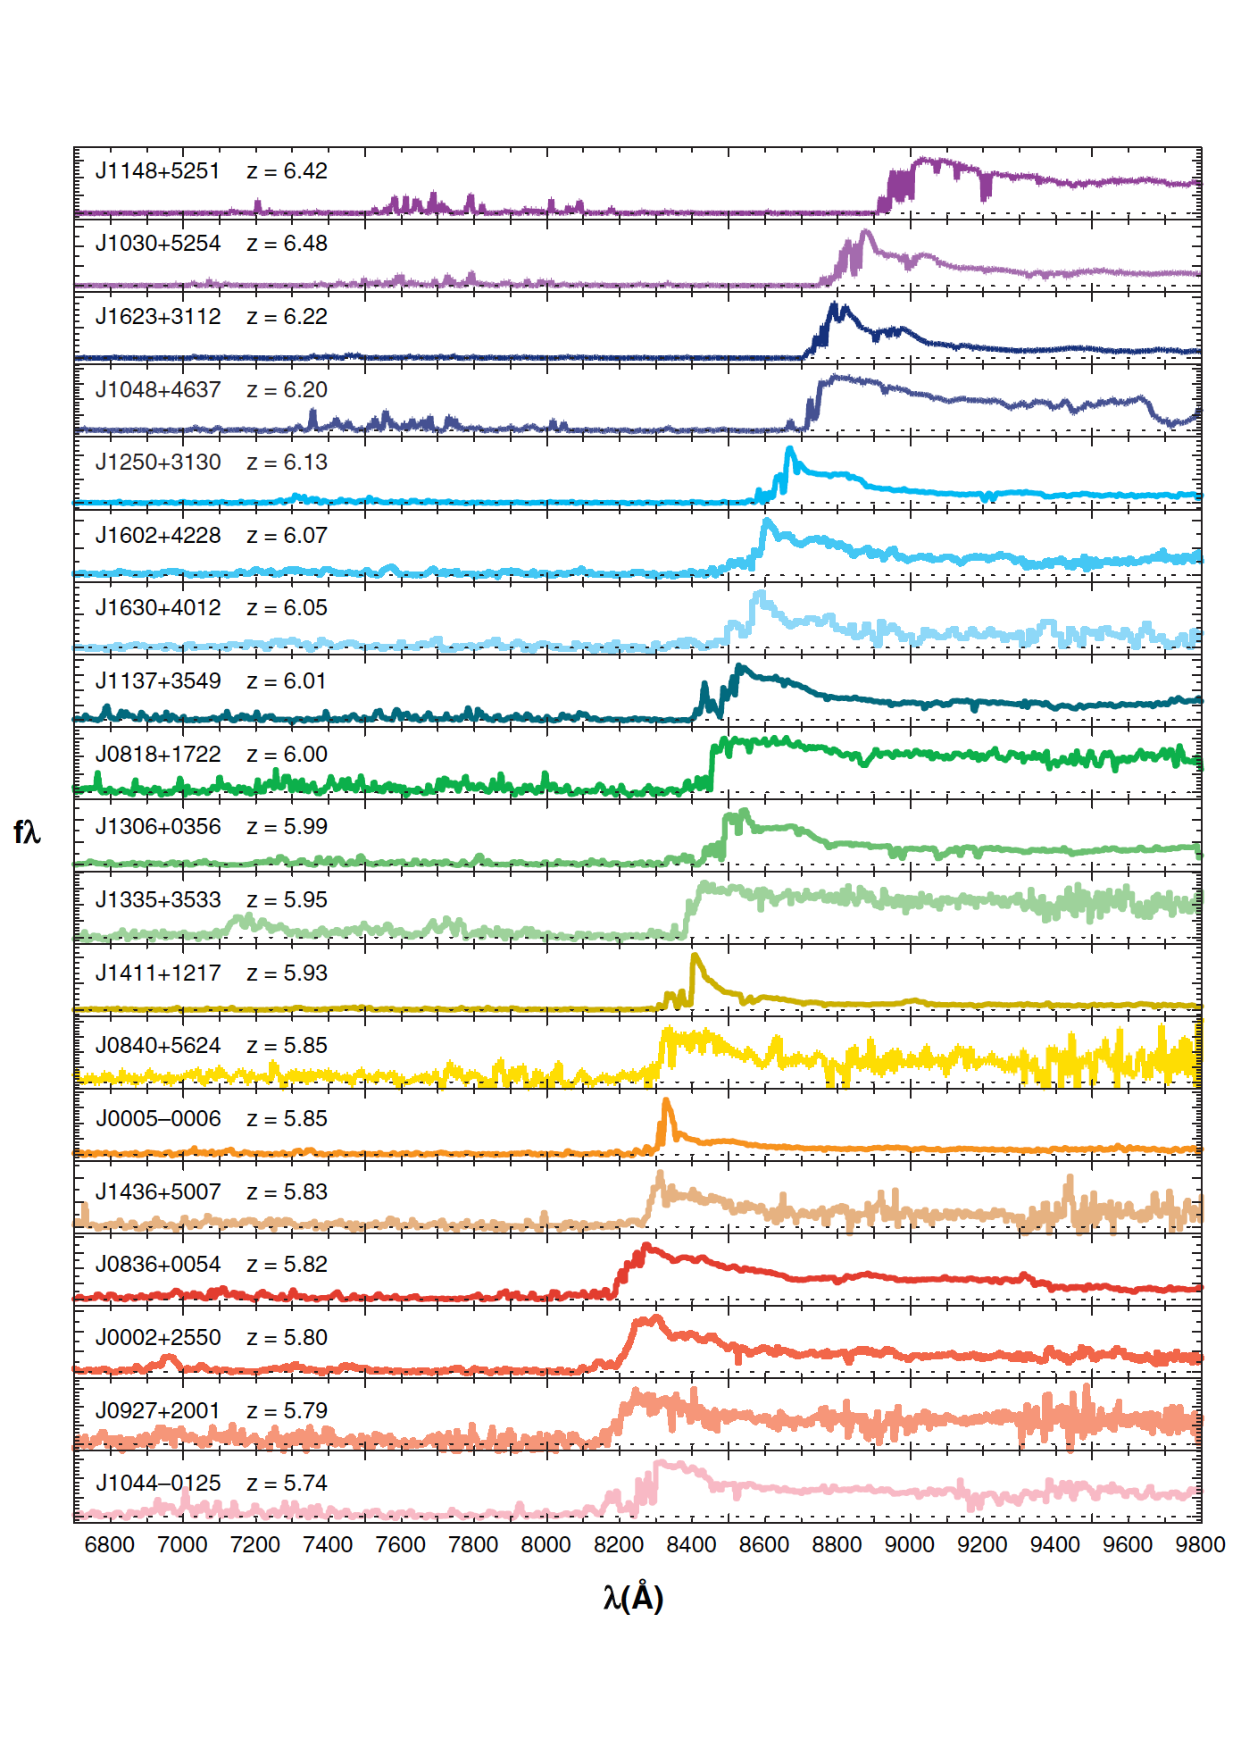
\includegraphics[width=.95\linewidth]{img/01/quasar_spectre.pdf} 
        \caption[Spectre de quasars]{Spectre de quasars à différents redshift présentant un tunnel Gunn Peterson.
        Ce tunnel devient plus important avec le redshift.
		Image extraite de \cite{fan_constraining_2006}.
 		\label{fig:spectre_quasar}}
\end{figure}



L’épaisseur optique traversée par les photons Lyman-alpha s'obtient à partir de ces spectres et de la formule suivante:
\begin{equation}
\tau_{GP} = \frac{\pi e^2}{m_e c} f_\alpha \lambda_\alpha H^{-1}(z) n_{HI},
\end{equation}
où $f_\alpha$ est la force d'oscillateur de la transition Lyman-alpha, $\lambda_\alpha = 1216 \AA$, $H(z)$ est la constante de Hubble, $n_{HI}$ la densité d'hydrogène neutre.
En appliquant cette formule aux différents spectres observés (figure \ref{fig:spectre_quasar}), \cite{fan_constraining_2006} ont mesuré la variation d'épaisseur optique en fonction du redshift.
Les résultats sont présentés sur la figure \ref{fig:epaisseur_optique_quasar}.
Il apparaît clairement que l'épaisseur optique augmente avec le redshift.



\begin{figure}
        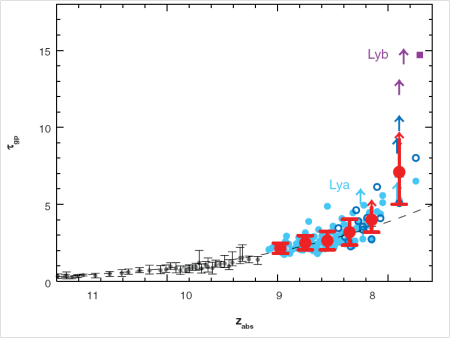
\includegraphics[width=.95\linewidth]{img/01/epaisseur_optique_quasar.png} 
        \caption[Epaisseur optique Lyman alpha]{%https://ism2009.wordpress.com/2009/04/28/on-the-density-of-neutral-hydrogen-in-intergalactic-space/
		Épaisseur optique calculée a partir des spectres de quasar de la Fig\,\ref{fig:spectre_quasar}
        Image extraite de \cite{fan_constraining_2006}.}
 		\label{fig:epaisseur_optique_quasar}
\end{figure}


Enfin, à partir de l'épaisseur optique, il est possible de déterminer la fraction d'hydrogène neutre traversée en supposant un modèle de photo-ionisation \citep{miralda-escude_reionization_2000}.
Une compilation des contraintes sur la fraction d'hydrogène neutre a été réalisée par \cite{2015ApJ...811..140B} et est présentée sur la figure \ref{fig:compile_constrains}.
On y observe une chute brutale dans la fraction de neutre à redshift $z\approx6$, représentant la fin de la période de réionisation.

\begin{figure}
        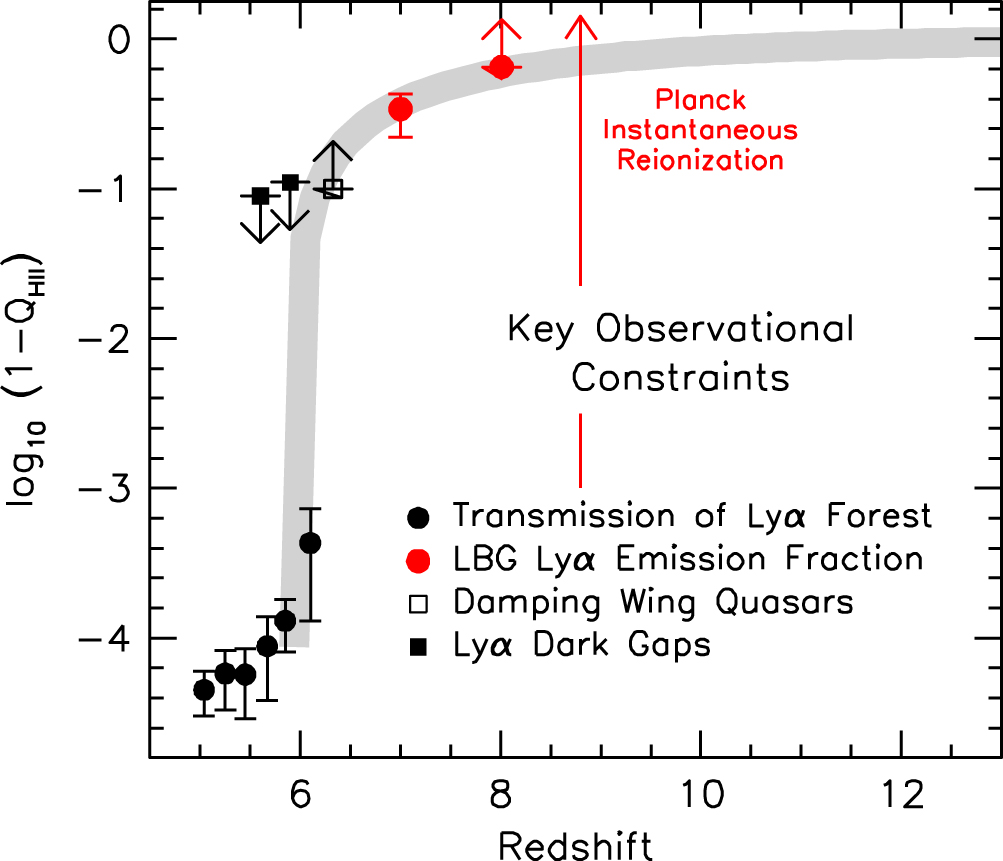
\includegraphics[width=.95\linewidth]{img/01/xionconstrains.jpg} 
        \caption[Fraction de neutre]{Fraction de neutre en fonction du redshift a partir d'observation Lymann-alpha.
        Compilation par \cite{2015ApJ...811..140B}}
 		\label{fig:compile_constrains}
\end{figure}


\subsection{CMB et épaisseur optique Thomson}

Une observation de la réionisation se trouve également dans les photons \ac{CMB}, car la réionisation constitue un avant-plan qui les a influencé. 
Les photons émis lors de la recombinaisons ont été diffusés, par le grand nombre d'électrons libérés pendant la réionisation.
Cette succession de diffusions Thomson, se traduit par une épaisseur optique qui sera calculée de la manière suivante : 

\begin{equation}
\tau_z = c \sigma_t \int_z^0 n_e (z) \frac{dt}{dz} dz,
\end{equation}
avec $\sigma_t$ la section efficace Thomson et $n_e (z)$ la densité d'électrons libres.

L'épaisseur optique Thomson cesse d'augmenter en dessous d'un certain redshift du à l’absence d'électrons libres permettant les diffusions.
Une représentation de cette contrainte, mesurée à partir des observations du satellite Planck se trouve sur la figure \ref{fig:epaisseur_optique_thomson}.
Différents modèles de réionisation y sont également présentés.
En utilisant un modèle de réionisation instantanée, \cite{planck_collaboration_planck_2016} estime le redshift de mi-réionisation à $z_r = 8.8 ^{+1.3}_{-1.2}$.

\begin{figure}
        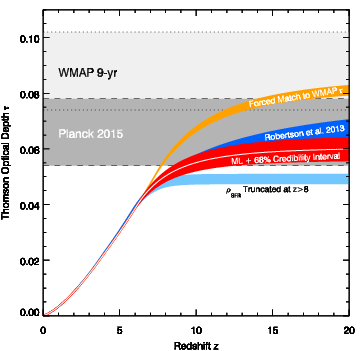
\includegraphics[width=.9\linewidth]{img/01/epaisseur_optique_thomson.png} 
        \caption[Epaisseur optique Thomson]{%https://inspirehep.net/record/1343310/plots
		Contrainte sur l'épaisseur optique Thomson.
        Image extraite de \cite{2015ApJ...802L..19R}
 		\label{fig:epaisseur_optique_thomson} }
\end{figure}



\subsection{Les futures observations}

%Dans un avenir proche, 
%Une des difficultés de l’étude de la période de réionisation est que celle ci a eu lieu tôt dans l'histoire de l'univers lors de son premier milliard d'années.
%Cette distance temporelle impose de regarder loin spatialement et donc de disposer de moyen observationnels important.

Observer la réionisation impose de disposer de moyens observationnels important.
Nous sommes encore au balbutiement des observations de la réionisation et une série de missions est en préparation.
Ces missions vont couvrir différentes parties du spectre, allant du radio avec l'observation de la raie à 21cm, aux rayons X pour la détection de quasars, en passant par les infrarouges pour étudier les galaxies.
Ces missions vont permettre d'obtenir une représentation complète de l'\ac{EoR} et compléter notre compréhension de la réionisation.
Parmi les missions qui vont livrer leurs résultats dans les années à venir on citera entre autre :

\paragraph{Raie à 21 cm :} % est émisse par les nuages d'hydrogène neutre.
\begin{itemize}
\item 2018 - SKA (Square-Kilometer Array) \href{https://skatelescope.org/}{site} 
\item 2016 - HERA (Hydrogen Epoch of Reionization Array) \href{http://reionization.org/}{site}
\end{itemize}

\paragraph{Galaxies :}

\begin{itemize}
\item 2019 - JWST (James Webb Space Telescope) \href{https://www.jwst.nasa.gov/}{site}
\item 2013 - ALMA (Atacama Large Millimeter Array) \href{http://www.eso.org/public/teles-instr/alma/}{site}
\end{itemize}

\paragraph{Quasars :}
\begin{itemize}
\item 2028 ATHENA (Advanced Telescope for High-ENergy Astrophysics)  \href{https://athena.cnes.fr/}{site}
\end{itemize}


%Une raie a 21 cm est émisse par les nuages d'hydrogène neutre.
%Lorsque que le spin de l'électron et du proton sont opposée, le niveau d'énergie de l'atome est légèrement supérieur au cas ou les spins sont alignés.
%Ces deux niveaux ont des énergies très proches et la transition est dite hyperfine.
%


%Lors du changement de spin d'un électron 
%
%\subsection{polarisation du CMB)}
%
%\subsection{fonction de luminosité UV}

%\section{Les futures observations}
%\subsection{SKA}
%\subsection{LOFAR}


\section{Influence de la réionisation sur la formation des galaxies}
\label{sec:refroidissement}

Nous avons vu en section \ref{sec:formationgalaxie} que la première étape de la formation des galaxies est la croissance des fluctuations primordiales.
Lorsqu'une sur-densité s’effondre, elle va entraîner avec elle une certaine quantité de gaz.
La seconde étape est donc d’effondrer ce gaz pour mettre en place la formation stellaire.
Or comme ce gaz est soumis à une compression, sa pression et sa température augmentent et s'opposent à la contraction.
L'effondrement des structures est alors limité : le refroidissement doit être efficace pour pouvoir continuer à effondrer le gaz (voir eg \cite{2004ARA&A..42...79B}).
Pour être en mesure de former des étoiles, un nuage de gaz doit avoir un temps dynamique :

\begin{equation}
t_{dyn} =\sqrt{\frac{3 \pi}{32 G \rho}},
\end{equation}
plus important que son temps caractéristique de refroidissement :
\begin{equation}
t_{cool} = \frac{3 nkT}{2 \Lambda(n,T)}.
\end{equation}

%\begin{equation}
%T_{vir} = \frac{\mu \Delta c}{6k_B} \left( G M_{vir} H_{(z)} \right)^{2/3}
%\end{equation}

\begin{figure}
        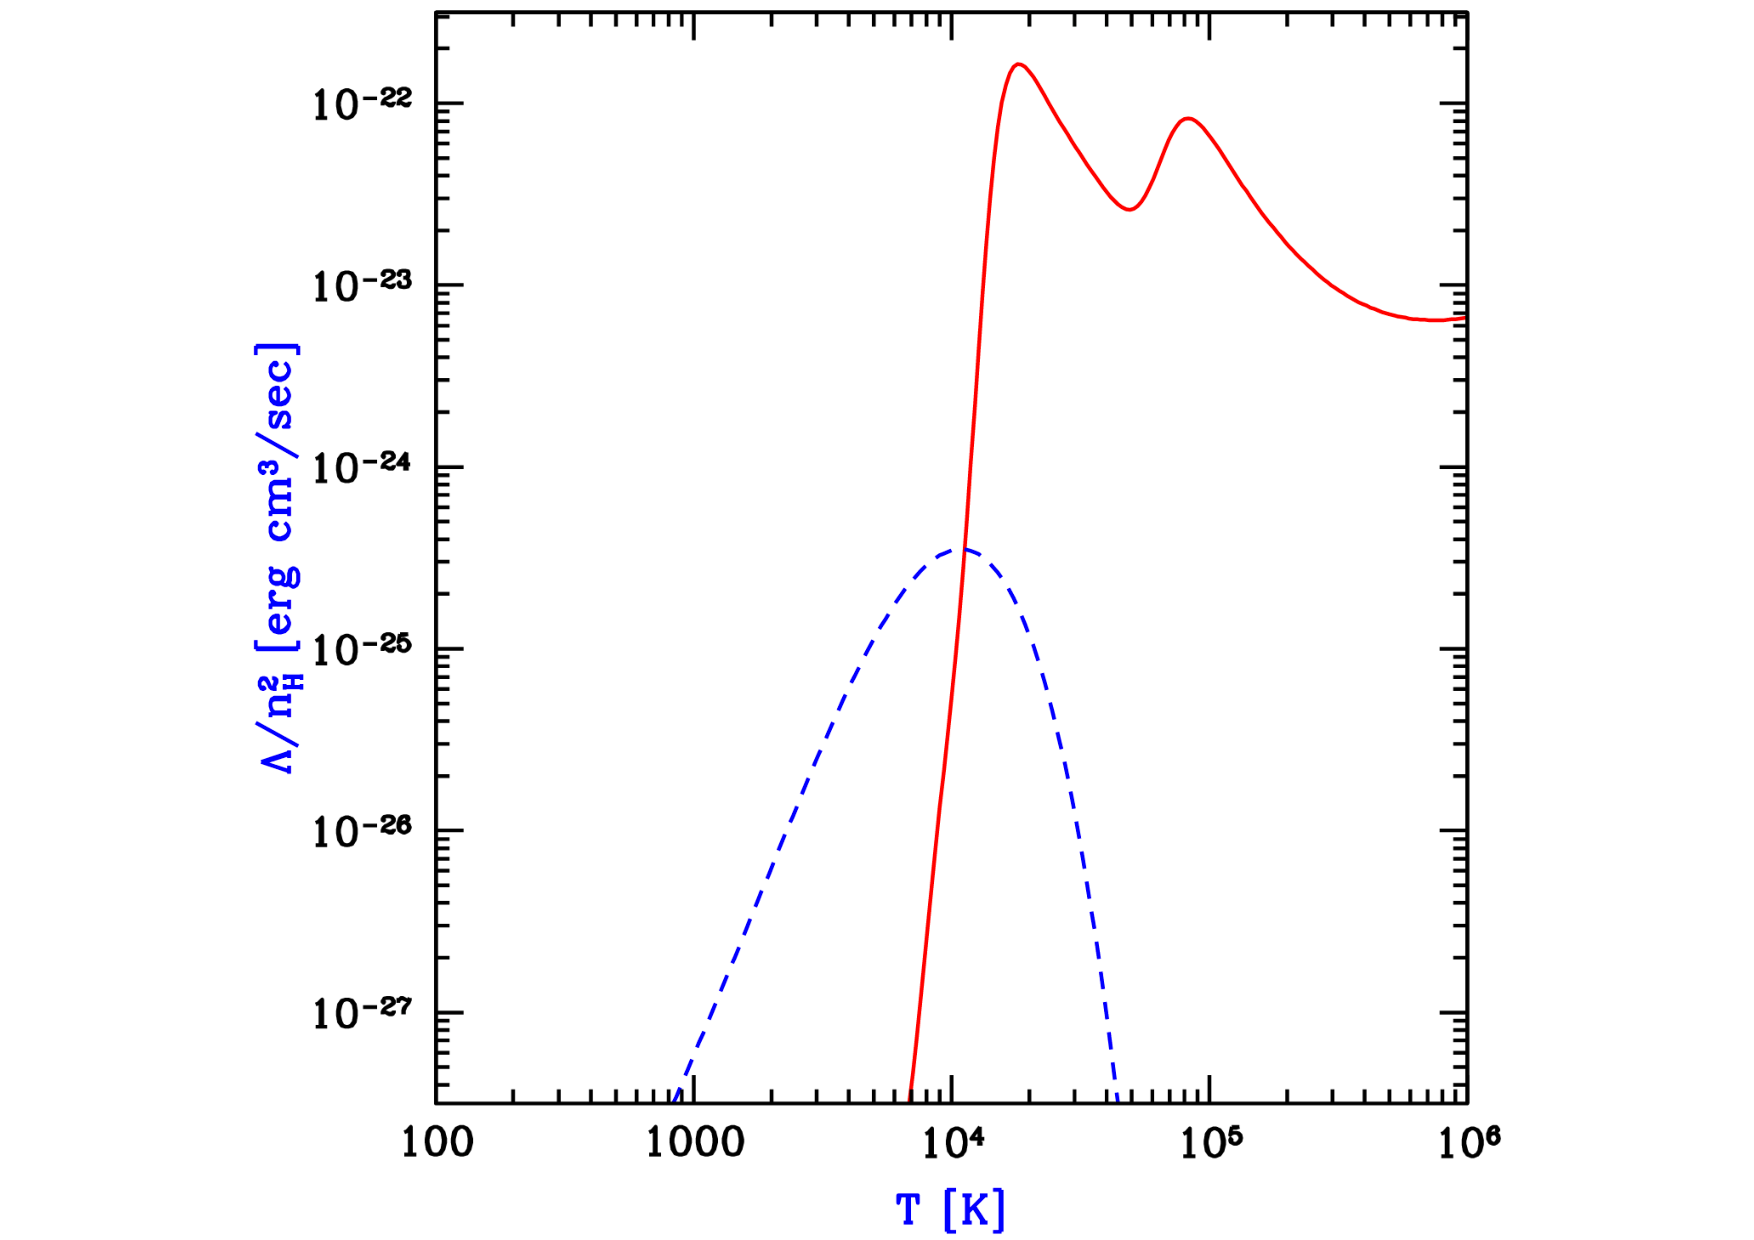
\includegraphics[width=.95\linewidth]{img/01/fonction_refroidissement.pdf} 
        \caption[Fonction de refroidissement]{Taux de refroidissement de l'hydrogène et de l'hélium atomique en rouge et moléculaire en bleu. 
        Figure extraite de \cite{2016PhR...645....1B}.
 		\label{fig:refroidissement}}
\end{figure}

Dans notre cas, le taux de refroidissement $\Lambda(n,T)$ est gouverné par l'émission de rayonnement de l'hydrogène atomique ou moléculaire et de l’hélium (voir figure \ref{fig:refroidissement}).
Ces rayonnements permettent de dissiper suffisamment d'énergie pour que l'effondrement puisse se poursuivre \citep{2001PhR...349..125B}.

Le type de processus de refroidissement majoritaire amène à distinguer les halos à refroidissement atomiques des halos à refroidissement moléculaire \citep{2002Sci...295...93A}.

\paragraph{Les halos à refroidissement moléculaire} auront une masse relativement faible ($M < 10^8 M_\odot$) et seront appelé "mini halo".
Leur importance dans le processus de réionisation est débattue \citep{2012ApJ...756L..16A} puisque la formation stellaire dans ces halos est gouvernée par la formation de $H_2$, or cette molécule est très sensible au rayonnement Lyman-Werner émis par les premières générations d'étoiles \citep{2002ApJ...575...49R}.
%demandant l'intro 
Ces halos n'ont pas été considérés dans cette étude.
%Je ne me suis pas intéressé à l'étude de ces halos durant ma thèse.

\paragraph{Les halos à refroidissement atomique} auront une masse plus importante ($M > 10^8 M_\odot$).
On distinguera cependant deux sous catégories : les halos massifs ($M > 10^9 M_\odot$) et les halos de faible masse ($M< 10^9 M_\odot$).
Ces derniers sont sensibles au photo-chauffage induit par le rayonnement UV \citep{1998ApJ...497...21M}.
Ces halos, voyant leur température augmenter vont également subir une augmentation de leur masse de Jeans (on parle alors de \textit{Jeans mass filtering}).
L'effondrement ne sera alors plus possible et la formation stellaire stoppée.
Puisque ce sont ces halos qui sont principalement impacté par la réionisation, un intérêt particulier sera porté sur les halos de masses $10^8 M_\odot < M< 10^9 M_\odot$ par la suite.
Les halos de masse $M > 10^9 M_\odot$ seront suffisamment massifs pour conserver leur capacité de refroidissement atomique, en écrantant le rayonnement UV.
%TODO plus sur les halos massifs.

\section{Physique de la réionisation}

Lorsqu'une étoile se forme dans un environnement d'hydrogène neutre, son rayonnement va être capable d'ioniser l'hydrogène autour d'elle dans une zone définie.
Ces zones forment des bulles, et quand plusieurs bulles apparaissent proches les unes des autre, elles percolent pour en former une plus grande.
Ces régions sont nommées régions HII et une grande partie de l'étude de l'\ac{EoR} consiste à étudier leurs croissances.

\subsection{Sphère de Strömgren}
\label{sec:stromgren}

Dans le but d’appréhender les principes de base à l’œuvre pendant la réionisation, nous allons commencer par nous placer dans le cas idéal d'une source unique.

Une source lumineuse ponctuelle apparaît instantanément dans un milieu infini, avec une densité et une température homogènes et composé exclusivement d’hydrogène neutre.

Les questions sont alors : 
\begin{itemize}
\item Comment va évoluer l’état d'ionisation du gaz autour de cette source ?
\item Quelle région cette source va ioniser autour d'elle?
\end{itemize}

En considérant l'équilibre entre $\dot{N_\gamma}$ le nombre de photons ionisant émis par la source et le taux de recombinaison du milieu, \cite{stromgren_physical_1939} a exprimé l'évolution du rayon  $r_i(t)$ de la sphère ionisée :

\begin{equation}
\frac{dr_i(t)^3}{dt} = -n_H \alpha_B(T)r_i (t)^3 + \frac{3 \dot{N_\gamma} }{4 \pi n_H},
\end{equation}

où $\alpha_B(T)$ est le coefficient de recombinaison, fonction de la température et $n_H$ la densité d'hydrogène neutre.
La solution de cette équation est de la forme :

\begin{equation}
r(t) = r_s \left( 1 - e^{-t\cdot \alpha_B(T) n_H } \right)^{1/3}
\end{equation}

%
%\begin{equation}
%t_{rec} = \left( \alpha_B(T) n_H \right) ^{-1}
%\end{equation}

Le rayon de Strömgren est défini comme étant la solution stationnaire de cette équation:

\begin{equation}
r_s = \left( \frac{3 \dot{N_\gamma} }{4 \pi \alpha_B(T) n_H^2} \right)
\end{equation}

Nous voyons ici que connaissant l'émissivité de la source et la densité et température du milieu environnant, il est possible d'estimer la taille de sa région HII.

\subsection{Le cas non idéal}

Nous venons de voir un modèle idéalisé sensé représenter la croissance des régions HII de manière individuelles, en réalité : 
\begin{itemize}
\item l'Univers est en expansion,
\item la densité n'est pas homogène,% (motif en papillon autour des filament)
\item les sources ne sont pas isolées,
\item l'intensité des sources n'est pas constante. %Les étoiles évoluent et meurent, si il n'y a 
\end{itemize}

Dune manière générale, l'évolution de la fraction d'hydrogène ionisée dans l'Univers, dépend de la balance entre le taux d'ionisation et le taux recombinaison \citep{0004-637X-514-2-648, RevModPhys.81.1405} :
\begin{equation}
\frac{dQ_{HII}}{dt} = \frac{\dot{N}_{ion}}{ <n_H>} - \frac{Q_{HII}}{t_{rec}}.
\label{eq:eqion}
\end{equation}

Cette relation fait intervenir le temps de recombinaison :

\begin{equation}
t_{rec} = \left( C\cdot \alpha^\beta <n_H> \left( 1+\frac{Y}{4X}\right) \left((1+z\right)^3  \right)^{-1}, 
\end{equation}

contenant l'information de la densité du milieu inter-galactique ou \ac{IGM} par le biais de $<n_H>$, de son inhomogénéité par l'intermédiaire du \textit{facteur de clumping} $C$ et de sa composition avec $X$ et $Y$ les fraction d'hydrogène et d'hélium.
Une grande partie de la difficulté de la modélisation de l'\ac{EoR} est contenue dans ce terme.

L'équation \ref{eq:eqion} fait également intervenir le taux d'émission de photons ionisants $\dot{N}_{ion}= \dot{n}_{ion} \cdot f_{esc}$, lui même fonction de $\dot{n}_{ion}$ le nombre de photons ionisants produit par les sources et de $f_{esc}$ la fraction d'échappement des photons. 
$f_{esc}$ caractérise directement le lien entre les photons ionisant produit par les sources et les photons qui vont être effectivement utiles à ioniser le milieu.
Elle contient une grande partie de la physique interne des galaxies.
%TODO devellope

$\dot{n}_{ion}$, le taux de production de photons ionisants, est directement fonction du taux de formation stellaire ou \ac{SFR}.
À partir de l'observation des fonctions de luminosités des galaxies à hauts redshifts (cf premier panneau de la figure \ref{fig:obs}), \cite{bouwens_reionization_2015} ont estimé l'histoire de formation stellaire ou \ac{SFH} durant la réionisation (cf second panneau de la figure \ref{fig:obs}).
On y observe une augmentation du nombre d'objets à forte luminosité UV avec le redshift, due à une augmentation de la formation stellaire induite par la croissance des structures.
Ce taux de formation stellaire constituera l'une des principales contraintes que l'on cherchera à reproduire lors de la réalisation de simulations.

%La figure \ref{fig:obs} présente les fonctions de luminosités des galaxies à haut redshift ainsi que les contraintes déterminées à partir de celles ci sur 
%Se sont les générations successives d'étoiles et l'augmentation du taux de formation stellaire qui permet a l'Univers de réioniser en entier.
%Le taux de production des photons est aussi fonction du profile d'émissivité des sources.
%Ce profil d’émissivité sera dépendant entre autre de la fonction de masse initiale




%taux d'effondrement des structures.

%l'Univers de réionise en entier car les sources sont nombreuses et c'est la percolation des régions HII des régions successives d'étoiles 

%Les régions HII croissent de manière asymétrique en fonction de la géométrie du milieu, et forment des motifs en "papillons" autour des amas et des filaments.
%La percolation de ces régions augmente petit à petit la fraction ionisée de l'Univers, jusqu'à ce qu'il ne reste plus que une fraction de neutre de l'ordre de $1-Q_{HII}=10^{-4}$.


\begin{figure}
		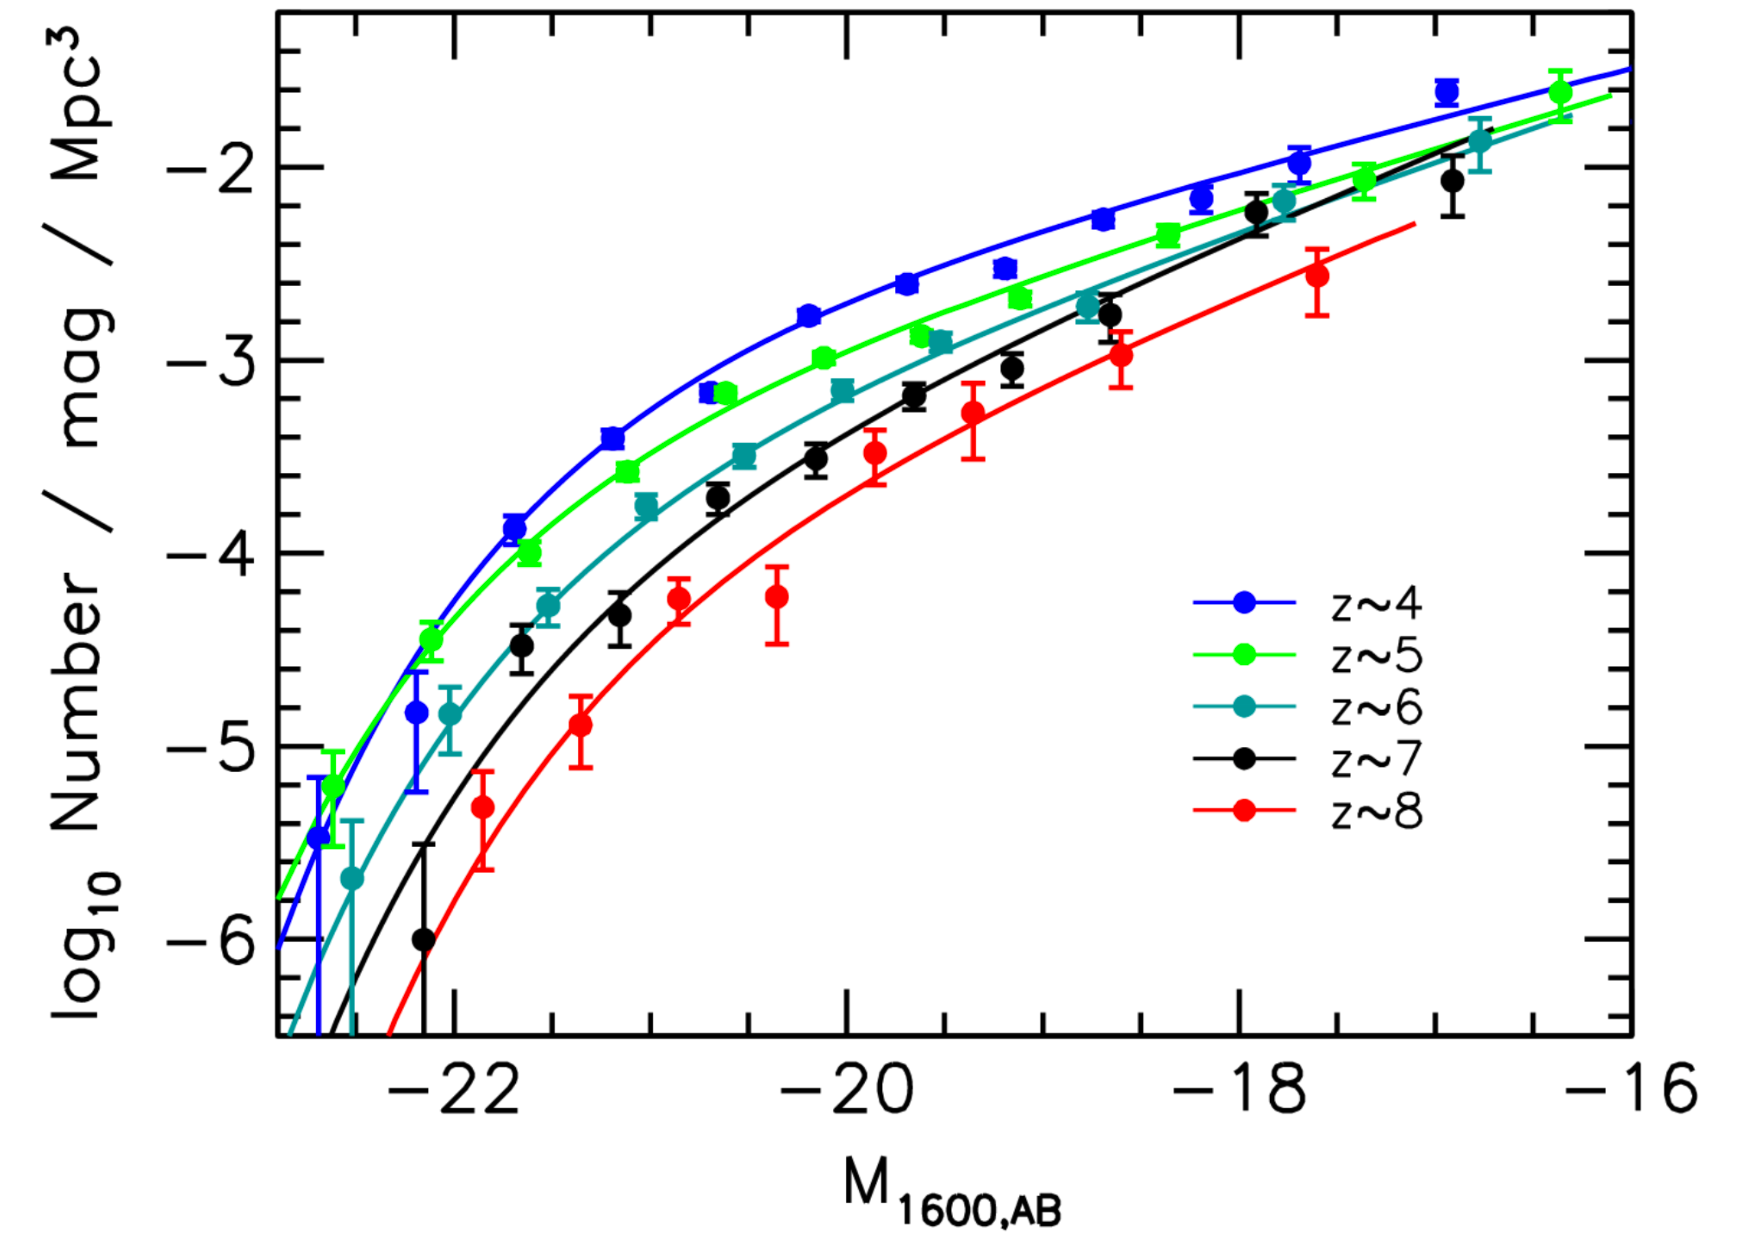
\includegraphics[width=.95\linewidth]{img/01/UV_lum_obs.pdf} 
        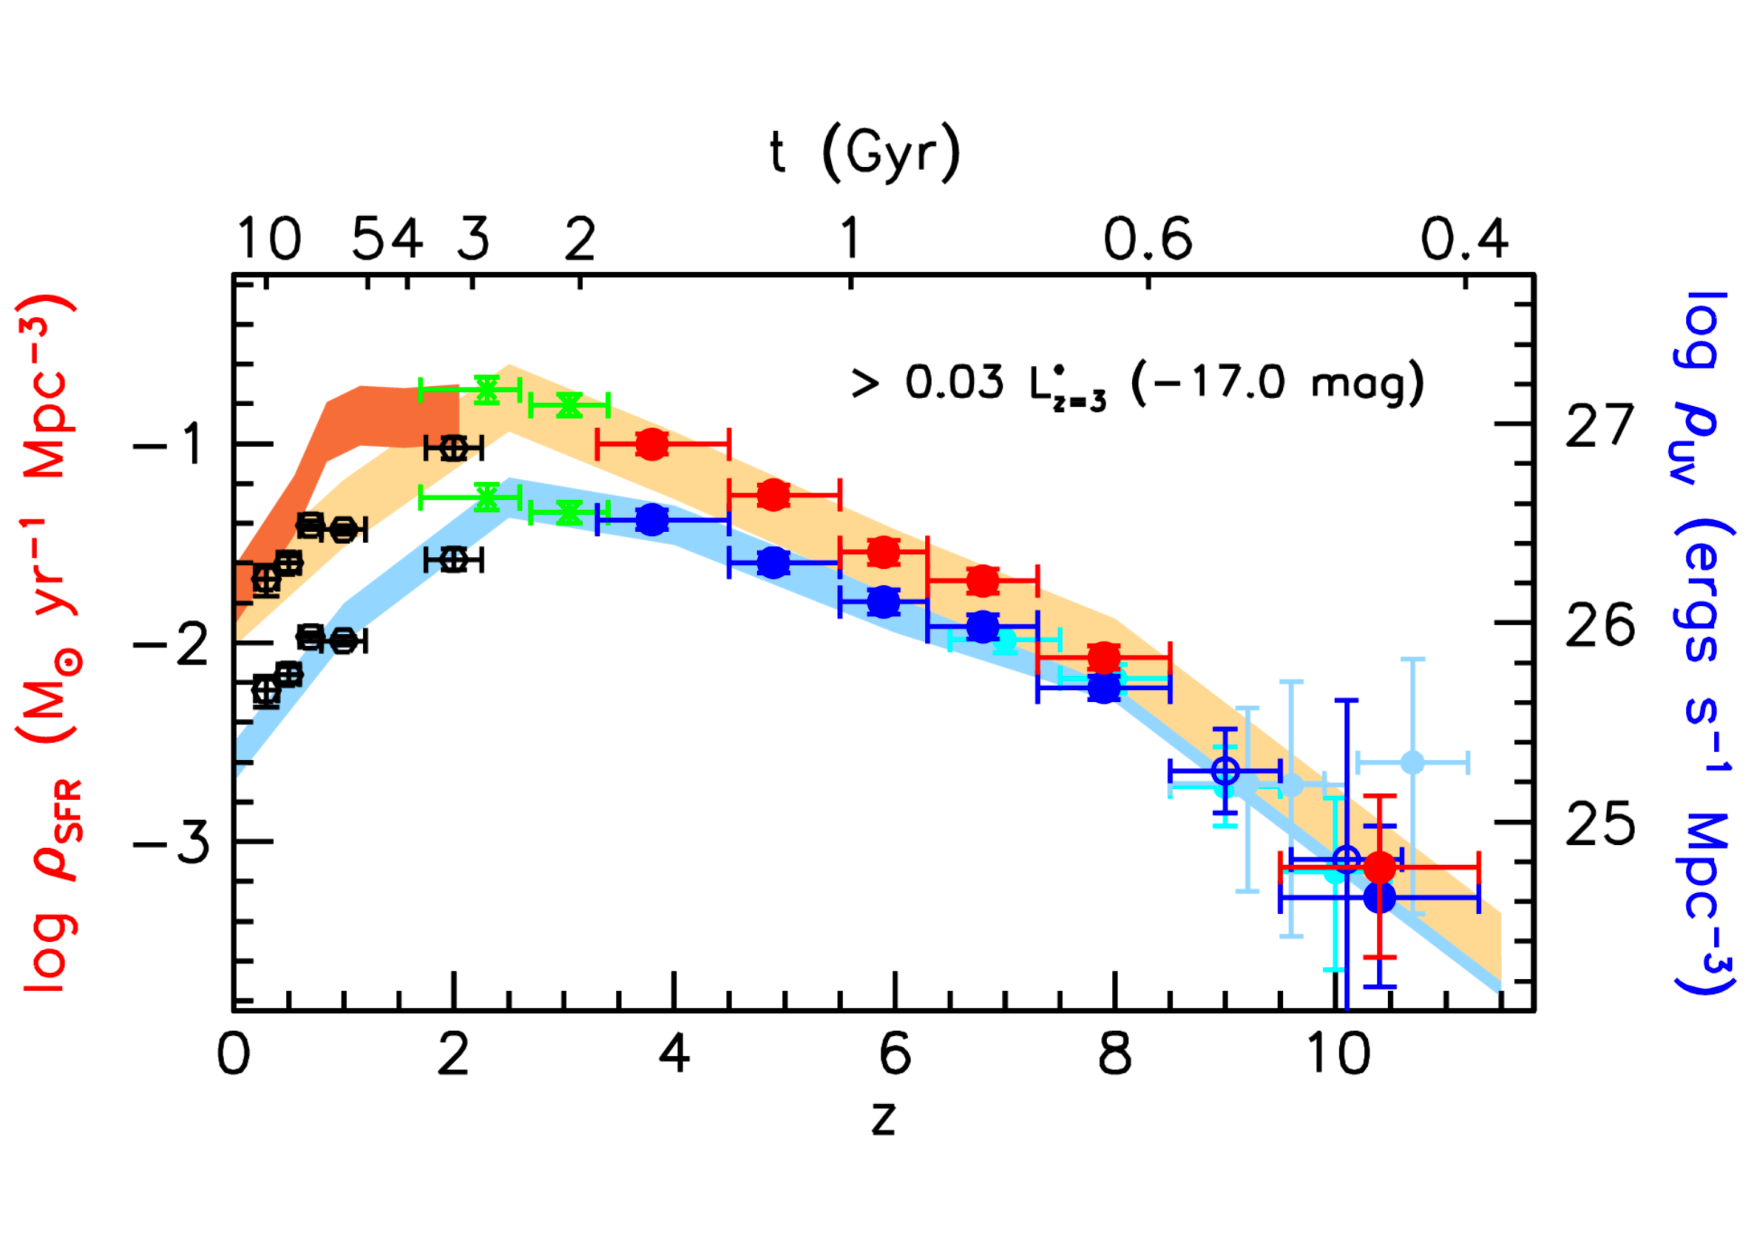
\includegraphics[width=.95\linewidth]{img/01/SFR_obs.pdf} 
        \caption[Contrainte SFH]{Haut: fonctions de luminosités à hauts redshifts. 
        Bas : contraintes observationnelles sur l'histoire de formation stellaire à hauts redshifts dérivées des fonctions de luminosités. 
        Figures extraites de \cite{bouwens_reionization_2015}.
 		\label{fig:obs}}
\end{figure}


On définira également le taux d'ionisation de l'hydrogène:
\begin{equation}
\Gamma = c \sigma n_\gamma
\end{equation}
où $\sigma$ est la section efficace de photo-ionisation de l'hydrogène, et $\gamma$ la densité numérique de photon ionisant.
%TODO develope
Il faudra donc que la formation stellaire ait produite suffisamment de photons pour réioniser tout l'Univers.
Des contraintes sur le taux de photo-ionisation ont été déterminées à partir d'observations par \cite{2013MNRAS.436.1023B} (voir figure \ref{fig:photoionisationrate}).
Il faut au minimum 1 photons ionisant par atomes, mais ce nombre est plus proche de 2 si l'on considère les effets liés à la recombinaison \citep{aubert_reionization_2010}.
Une fois l'Univers réionisé, celui ci baigne dans un fond UV uniforme \citep{haardt_radiative_2012}.

%$ <n_H>$ est la densité moyenne d'Hydrogène dans l'Univers, comme il dépend de $a$, ce terme contient l'information de l'expansion de l'Univers.

\begin{figure}
        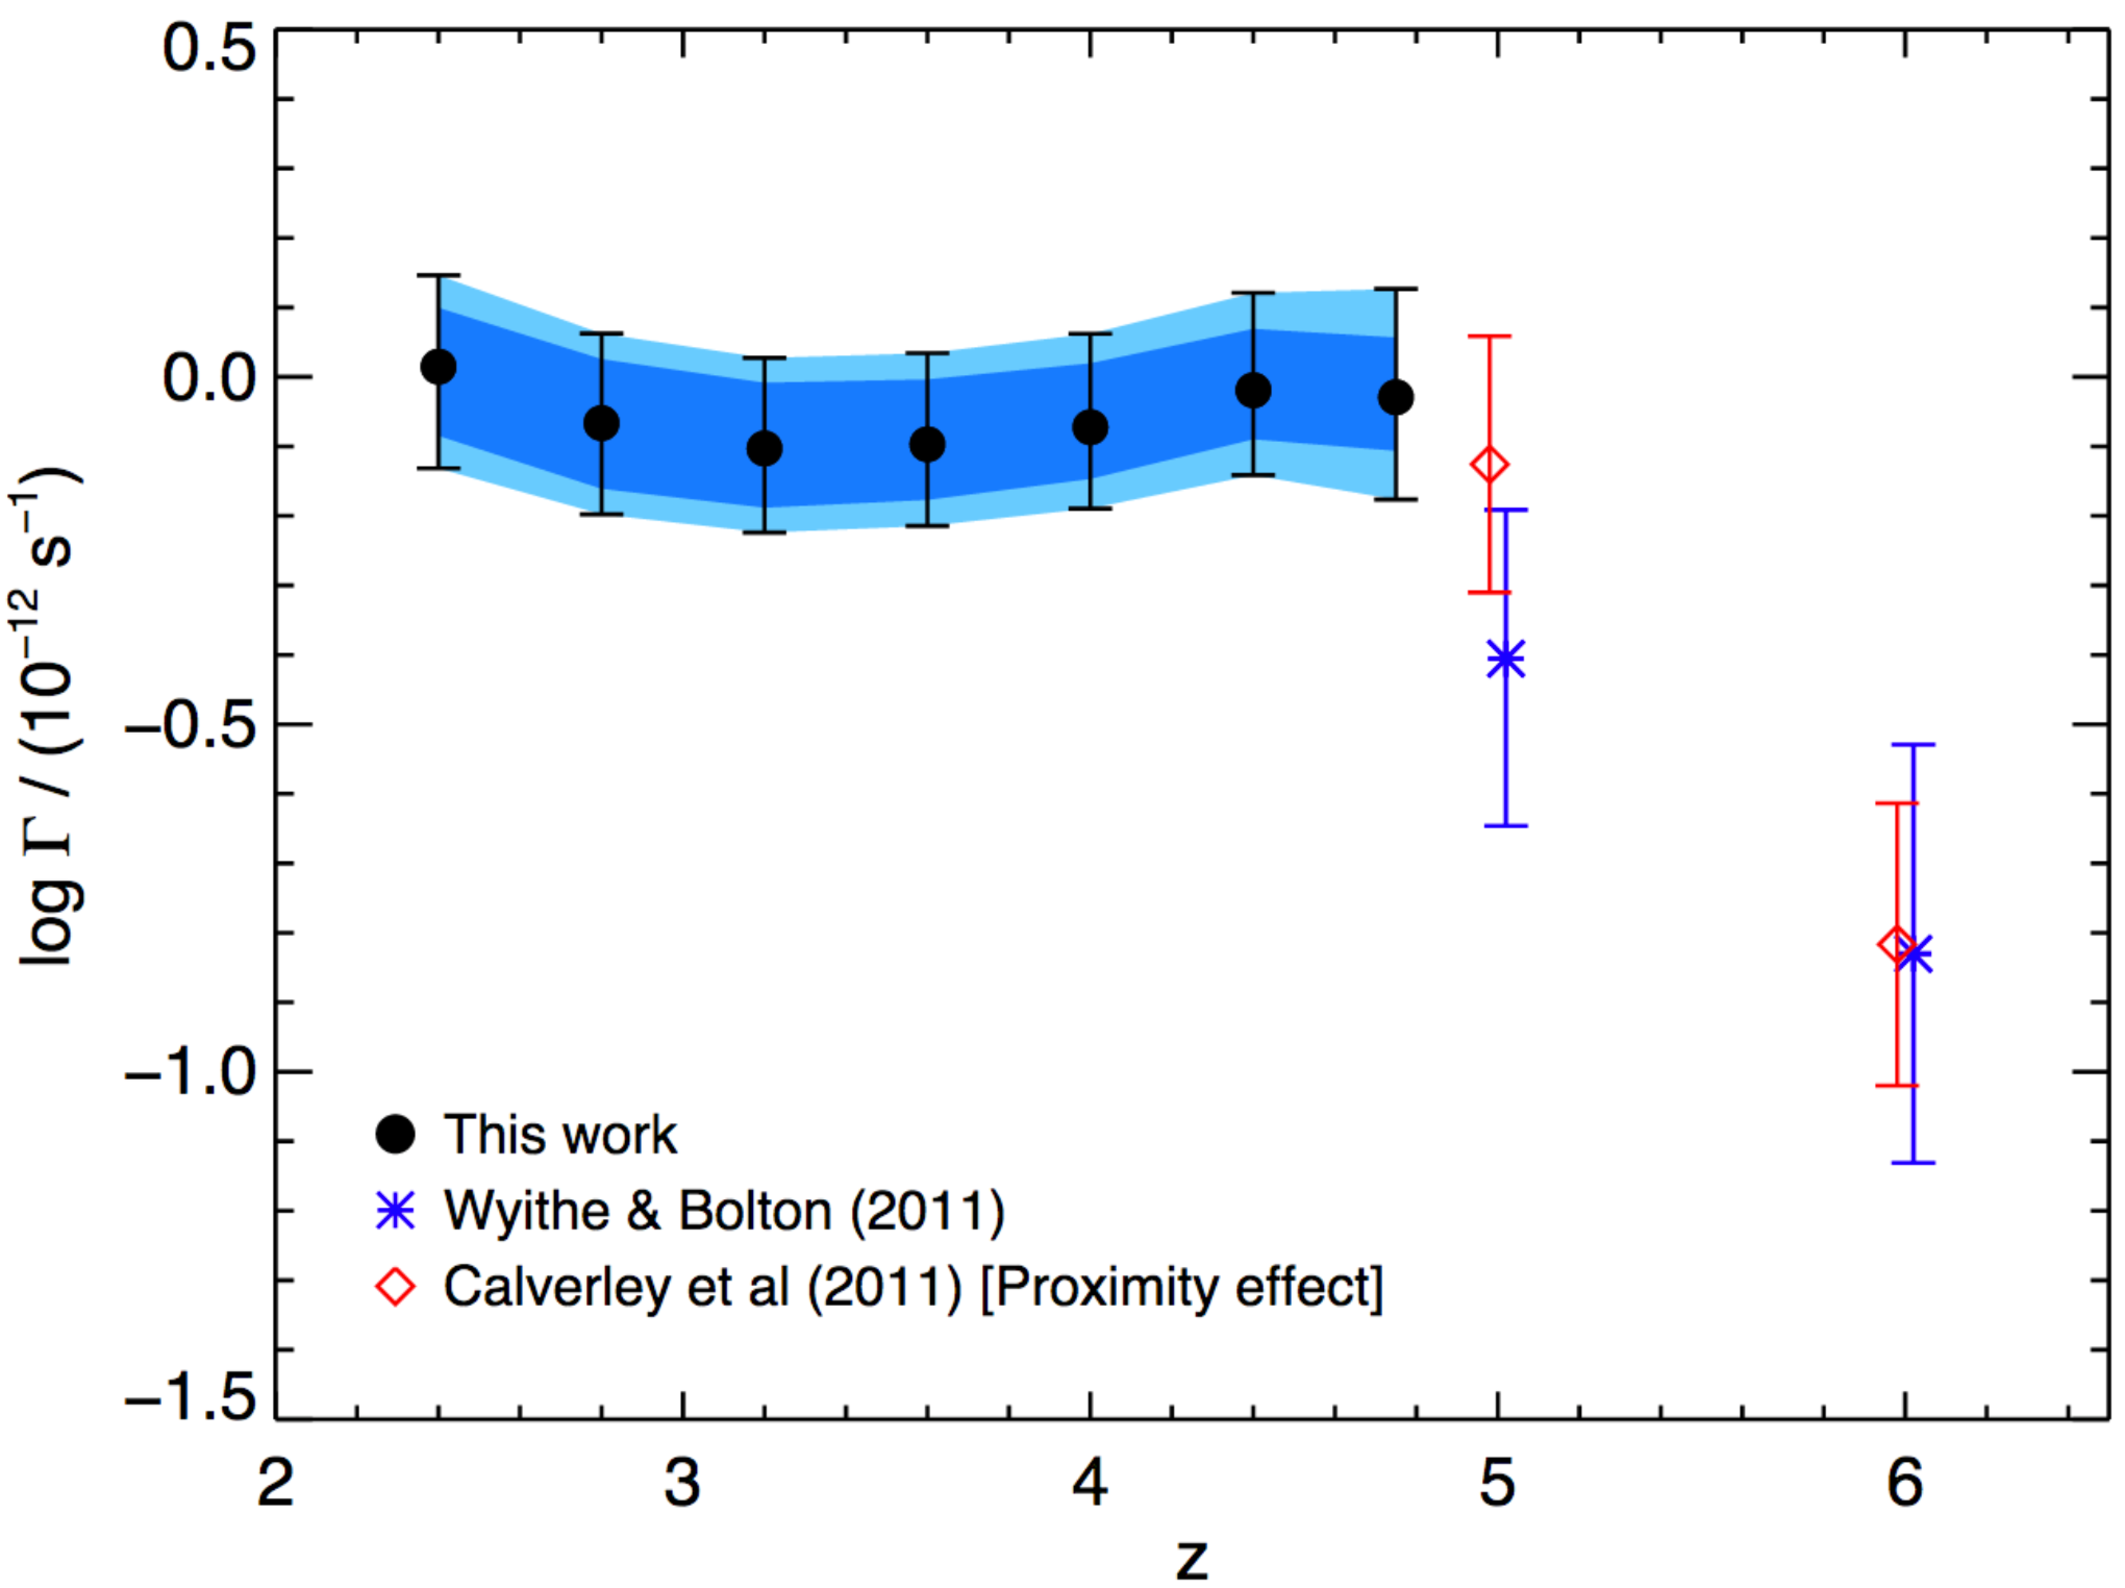
\includegraphics[width=.95\linewidth]{img/01/photon_obs.pdf} 
        \caption[Taux de photo-ionisation ]{Contraintes observationnelles sur le taux de photo-ionisation de l'\ac{IGM} en fonction du redshift. 
        Figure extraite de \cite{2013MNRAS.436.1023B}.
 		\label{fig:photoionisationrate}}
\end{figure}



\clearpage


%\section{Quelques questions en suspens}
%
%%quand est ce arrivé?
%%quelles sont les sources? -> débat galaxies vs quasars
%
%%En utilisant la halo mass function presenté en TODO REF, 
%
%La provenance des photons qui ont réionisé l'Univers est toujours indéterminée.
%En étudiant la répartition du nombre de galaxies en fonction de leurs masses, on observe que les galaxies les moins massives sont nombreuse et que les galaxies les plus massives sont rare.
%Or, plus une galaxie est massive, plus celle ci va créer des étoiles, et donc eméttres des photons.
%La balance entre les nombreuses galaxies peu lumineuses, et les rare galaxies extrêmement lumineuse reste à déterminer.
%
%De plus, les quasars, objets extrêmement lumineux, situé dans les galaxies les plus massives, augmente encore le budget de photon.
%Les quasars ont contribué à réioniser l'Univers mais dans quelles proportion?
%La figure \ref{fig:gal_AGN} présente le budget de photon plausible pour les galaxies ou les quasars selon \cite{trac_computer_2011}.
%Il faut un certain temps pour mettre en place les conditions propices à l'apparition d'un quasar, est ce que ce temps a été suffisant avant z=6, pour en former suffisamment ?
%Certain travaux soutiennent que c'est le cas (eg \cite{chardin_large-scale_2017}) cependant seul le rayonnement provenant des galaxies a été considérer lors de cette thèse.
%
%Si ce sont les galaxies qui ont réionisé l'Univers, quelle est le ratio entre la quantité de rayonnement produite et la quantité de rayonnement capable d'atteindre l'\ac{IGM}?
%La fraction d'échappement ($f_{esc}$) permet de faire le lien entre les observations et la physique réellement en place au sein des galaxies.
%Elles dépend de nombreux paramètres comme la formation stellaire ou les propriétés du milieu.
%Comment évolue t-elle en fonction de la masse des galaxies? 
%
%\begin{figure}
%        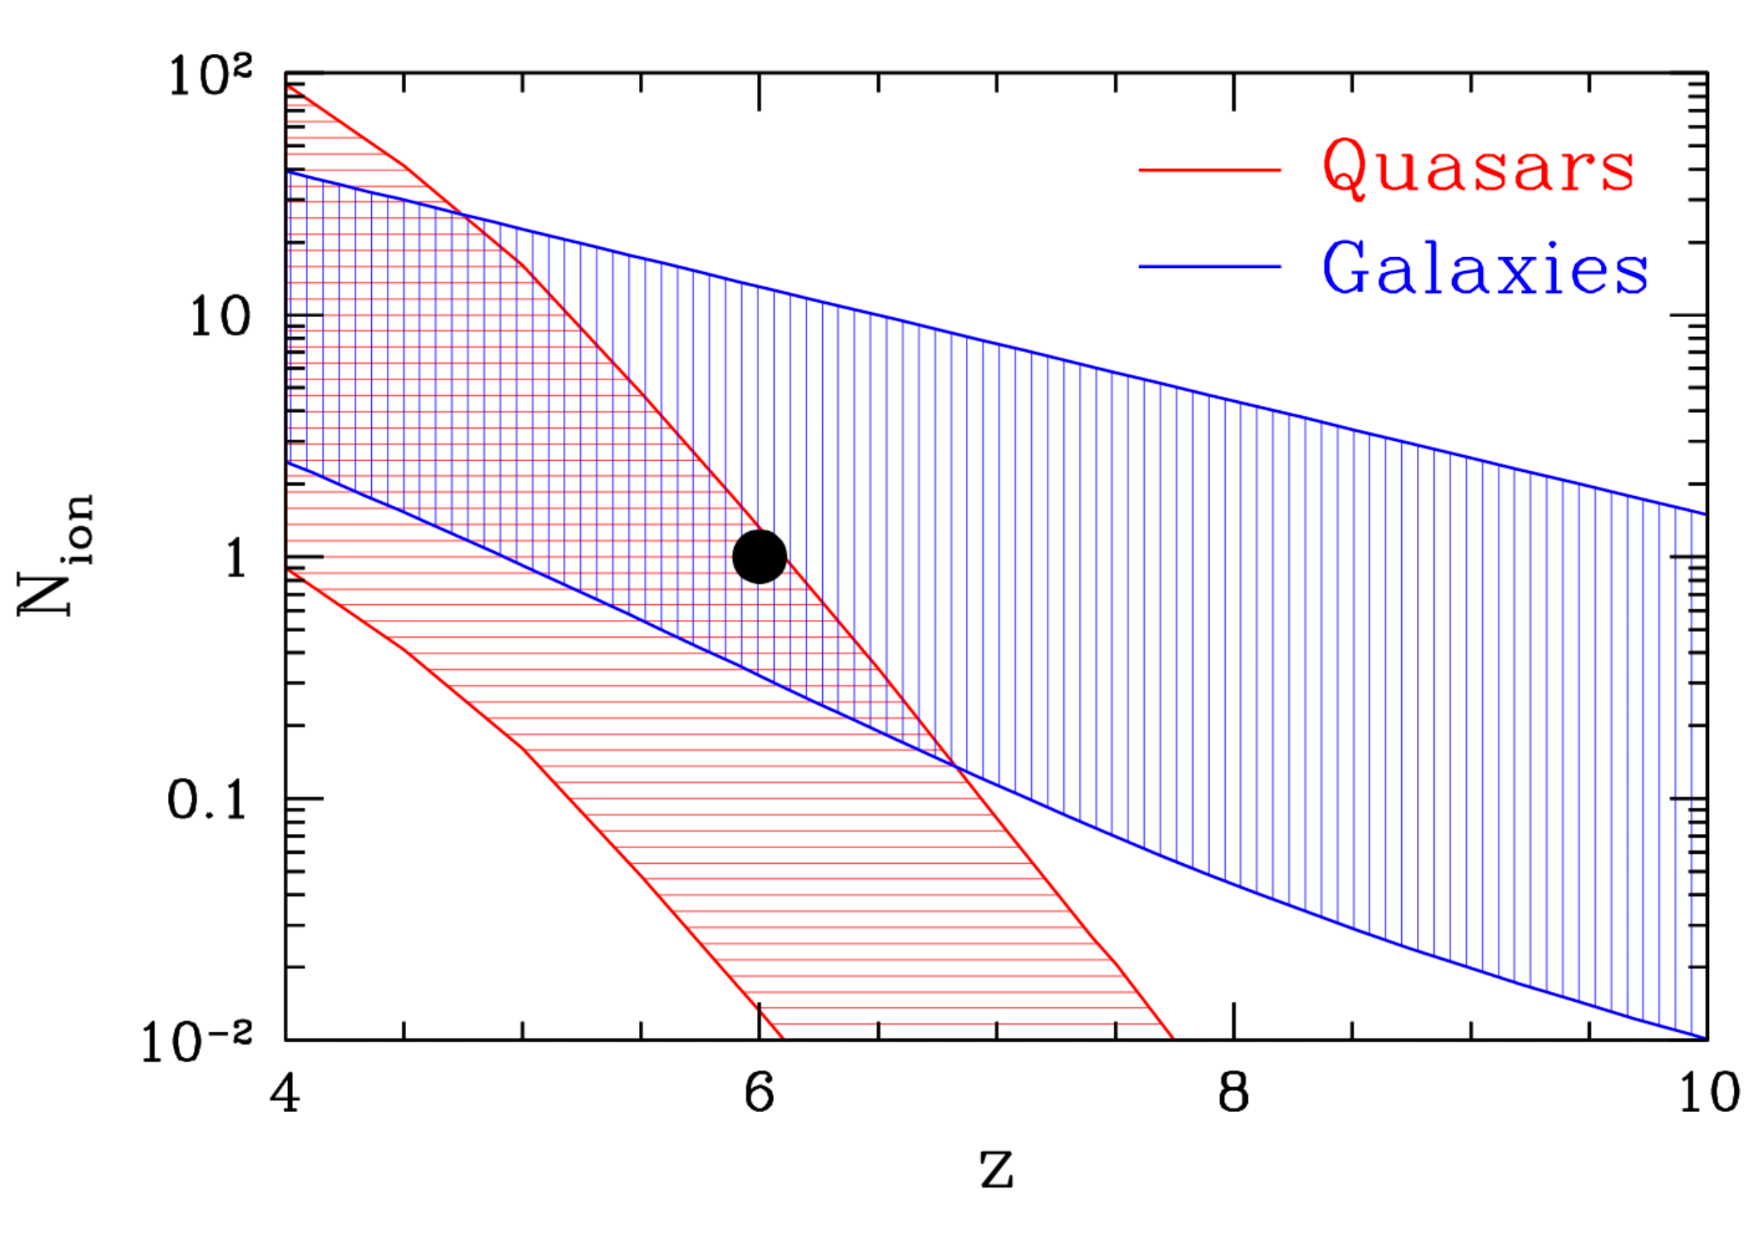
\includegraphics[width=.9\linewidth]{img/01/gal_AGN.pdf} 
%        \caption{Budget de photons provenant des galaxies et des quasars durant la reionization selon \cite{trac_computer_2011}.
% 		\label{fig:gal_AGN} }
%\end{figure}
%
%%outlier dans l'épaisseur optique des quasars
%%Le groupe local ?
%%Le développement d’expériences destinées entre
%%autres le signal à 21 cm de la réionisation comme 
%

